
\documentclass[a4paper,14pt]{extarticle}
\usepackage{cmap}
\usepackage[T2A]{fontenc}
\usepackage[utf8]{inputenc}
\usepackage{setspace}
\usepackage{titlesec}
\usepackage{diagbox}
%\renewcommand{\baselinestretch}{1.5}
\onehalfspacing
\usepackage[english,russian]{babel}
\usepackage{comment}
\usepackage{amsmath,amsfonts,amssymb,mathtext,cite,enumerate,float,indentfirst,floatflt}

\usepackage[left=3cm,right=1cm,
    top=2cm,bottom=2cm,bindingoffset=0cm]{geometry}
		
\renewcommand{\refname}{whatever}	
		
\usepackage{multicol,subcaption,multirow}
\usepackage{graphicx,caption,tocvsec2}

\addto\captionsrussian{\def\refname{СПИСОК ИСПОЛЬЗОВАННЫХ ИСТОЧНИКОВ}}

\usepackage{fancyhdr,fancybox}
\graphicspath{{images_errors_CS/}{images_additional/}{images_errors_EL/}}
\pagestyle{plain}
\fancyhead[L]{\thepage}
\renewcommand{\headrulewidth}{0pt}

\captionsetup[subfigure]{labelformat=simple, labelsep=colon}
\renewcommand{\thesubfigure}{\alph{subfigure}}

\titleformat*{\section}{\large\bfseries}
\titleformat*{\subsection}{\normalsize\bfseries}

\makeatletter
\renewcommand*{\@alph}[1]{%
  \ifcase#1\or а\or б\or в\or г\or
    д\or е\or ё\or ж\or з\or и\or й\or
    к\or л\or м\or н\or о\or п\or р\or с\or\v т\or
    у\or ф\or х\or ц\or ч\or ш\or щ\or ъ\or ы\or ь\or э\or ю\or \v я\else\@ctrerr\fi
}
\makeatother

\begin{document}

\section{Метод декомпозиции Шварца. Одномерный случай.}

Расмотрим в заданной расчётной области $\Omega=[r_1, r_2]$ дифференциальное уравнение равновесия для трубы, записанное в матричном виде:
\begin{equation}\label{SLAUStandart}
\textbf{Ku}=\textbf{f}.
\end{equation}
Разобъем область $\Omega$, для примера, на две пересекающиеся подобласти: $\Omega=\cup_{i=1}^{2} \Omega_{i}$, где $\Omega_1=[r_1, r_3]$ и $\Omega_2=[r_4, r_2]$ ($r_1$ и $r_2$ - внешние границы, $r_4$ и $r_3$ - внутренние границы). Обозначим начальное линейное приближение как $u^0$.

(Здесь будет рисунок разбиения)

Для начала, решаем задачу, записанную в матричной форме, в области $\Omega_{1}$:
\begin{equation}
K_{\Omega_{1}} u^{n+\frac{1}{k}} = f^{n+\frac{1}{k}}
\end{equation}
с кинематическим граничным условием на границе $r_1$
\begin{align*}
u(r_1)=u^0 
\end{align*}
и силовым граничным условием на границе $r_1$
\begin{equation}
\sigma_{r_1}=p_{r_1},
\end{equation}
где $k$ - количество подобластей (в нашем случае k=2). 

Следующим шагом решим задачу, записанную в матричной форме, в области $\Omega_{2}$:
\begin{equation}
K_{\Omega_{2}} u^{n+\frac{2}{k}} = f^{n+\frac{2}{k}}
\end{equation}
с кинематическим граничным условием на границе $r_4$
\begin{align*}
u(r_4)=u^{\frac{1}{2}} в \Omega_1
\end{align*}
и силовым граничным условием на границе $r_2$
\begin{equation}
\sigma_{r_2}=p_{r_2},
\end{equation}
где $k$ - количество подобластей (в нашем случае k=2). 
Дальнейший итерационный процесс решения дифференциального уравнения 
\begin{equation}
K_{\Omega_{i}} u^{n+\frac{i}{k}} = f^{n+\frac{i}{k}}, \  i=1,\ldots,k
\end{equation}
где k -количество подобластей, продолжается до тех пор, пока выполняется условие
\begin{equation}
\sqrt{\sum_{i=1}^{n} \dfrac{ (u^{n+1}-u^{n})^2}{ (u^{n+1})^2 }\dfrac{s_{i}}{\sum{s_i}}}
\end{equation}
где $u^{n+1}$ - численное решение, полученное по прошествию одного расчёта итерационного процесса, $u^{me}$ - численное решение, полученное на прошлой итерации, $s_i$ - полусумма двух шагов $\dfrac{h_i+h_{i+1}}{2}$, $\sum{s_i}$ - сумма всех шагов на всём отрезке.  


\newpage
\section{Результаты решения задачи для упругой трубы. Одномерный случай.}

Рассмотрим случай, когда внутреннее давление $p_a=20$ МПа, внешнее давление $p_b=0$ МПа. Тогда аналитическое радиальное перемещение считается по формуле :
\begin{equation}\label{perem}
u=\frac{\left(1-2\nu\right)\left(1+\nu\right)}{E} \frac{p_a a^2}{b^2-a^2}r+\frac{1+\nu}{E}\frac{a^2 b^2}{r}\frac{p_a}{b^2-a^2}.
\end{equation}

Вычисление аналитического радиального напряжения производится по формуле :
\begin{equation}
\sigma_{rr}=\frac{p_a a^2}{b^2-a^2}-\frac{a^2 b^2}{r^2}\frac{p_a}{b^2 -a^2}
\end{equation}

Вычисление аналитического окружного напряжения производится по формуле :
\begin{equation}
\sigma_{\varphi\varphi}=\frac{p_a a^2}{b^2-a^2}+\frac{a^2 b^2}{r^2}\frac{p_a}{b^2 -a^2}
\end{equation}	

Для решения поставленной задачи примем, что материал цилиндра имеет следующие параметры: модуль Юнга $E - 70000 \:\text{МПА}$ и коэффициент Пуассона $\nu=0.34$. Внутренний радиус цилиндра $a - 10 \:\text{мм}$, внешний радиус цилиндра $b - 20 \:\text{мм}$.

Расчёт относительной погрешности произведён по формуле для нормы, являющейся конечномерным аналогам следующих пространства $L_2$:
\begin{equation}\label{Error_Ot_L2}
\sqrt{\sum_{i=1}^{n} \dfrac{ (u_i^{an}-u_i^{me})^2}{ (u_i^{an})^2 }\dfrac{s_{i}}{\sum{s_i}}}
\end{equation}
где $u^{an}$ - аналитическое решение, $u^{me}$ - численное решение, $s_i$ - полусумма двух шагов $\dfrac{h_i+h_{i+1}}{2}$, $\sum{s_i}$ - сумма всех шагов на всём отрезке. 
\\
Коэффициент относительного захлёста (Overlapping coefficient) - 0.24. Критерий останова - $10^{-4}$.

\begin{tabular}{|l|c|c|c|c|}\hline
\diagbox[width=10em]{Кол-во\\подобластей}{Критерий\\ останова \varepsilon}&
  10^{-3} & 10^{-4} & 10^{-5} & 10^{-6} \\ \hline
2 & 59 & 92 & 124 & 157 \\ \hline
4 & 205 & 387 & 576 & 765 \\ \hline
10 & 609 & 1691 & 3062 & 4473 \\ \hline
\end{tabular}

Проведена серия расчётов на сетке N=100. Результаты расчётов представлены ниже. 

\begin{figure}[h]
\begin{center}
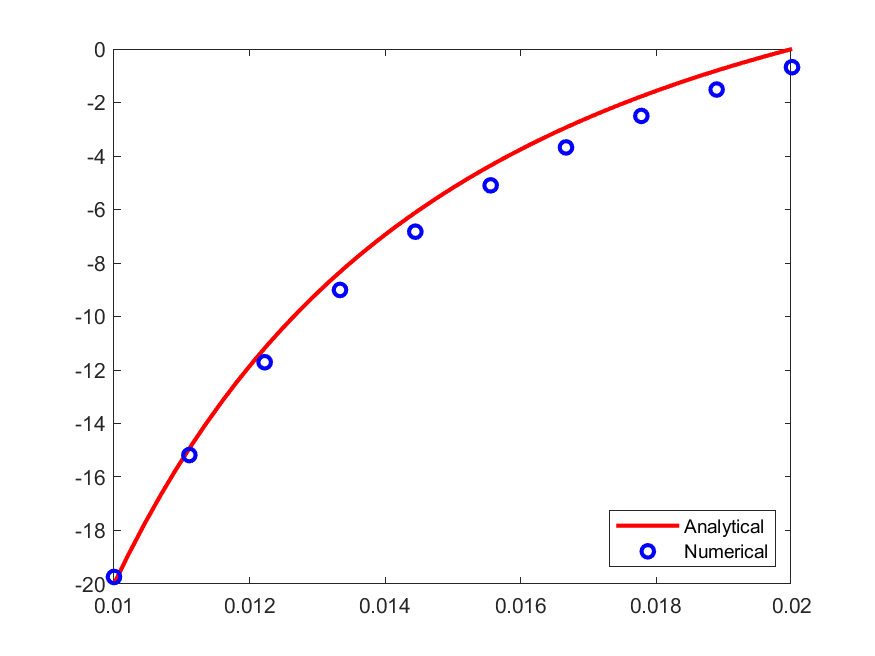
\includegraphics[width=95mm]{graphs/SigmaR.png}
\caption{Зависимость радиальных напряжений от радиуса}
\label{1r}
\end{center}
\end{figure}


\begin{figure}[h]
\begin{center}
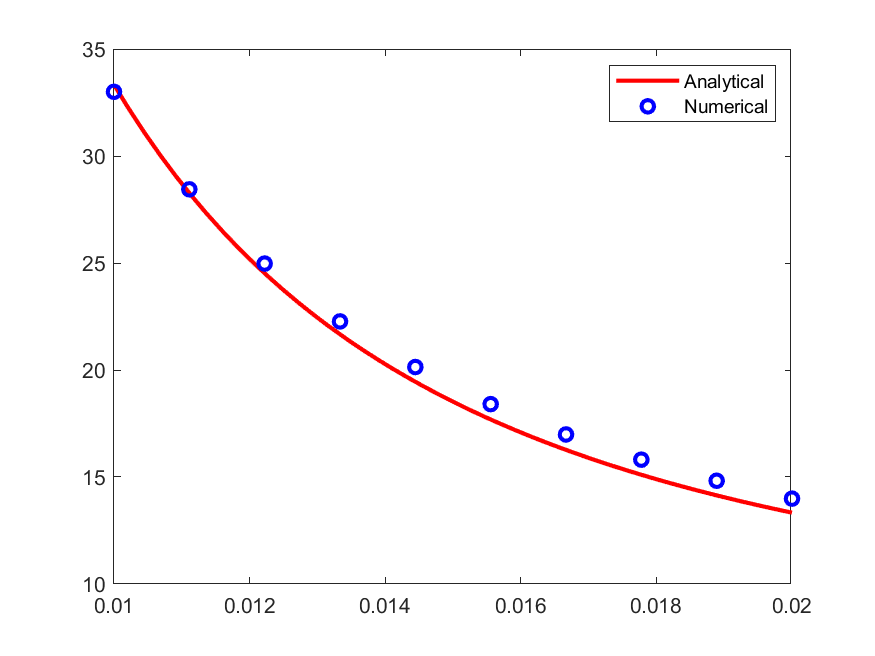
\includegraphics[width=95mm]{graphs/SigmaT.png}
\caption{Зависимость окружных напряжений от радиуса}
\label{1t}
\end{center}
\end{figure}

\begin{table}
\caption{Относительная радиальная погрешность , пространство $L_2$}
\begin{tabular}{|l|c|c|c|}\hline
\diagbox[width=10em]{Кол-во\\подобластей}{Сетка}&
  50 & 100 & 200 \\ \hline
1 & 2.72$\times 10^{-2}$ & 1.36$\times 10^{-2}$ & 6.78$\times 10^{-3}$ \\ \hline	
2 & 2.65$\times 10^{-2}$ & 1.33$\times 10^{-2}$ & 6.61$\times 10^{-3}$ \\ \hline
4 & 2.53$\times 10^{-2}$ & 1.21$\times 10^{-2}$ & 5.57$\times 10^{-3}$ \\ \hline
10 & 1.62$\times 10^{-2}$ & 1.05$\times 10^{-2}$ & 9.53$\times 10^{-3}$ \\ \hline
\end{tabular}
\end{table}

\begin{table}
\caption{Относительная окружная погрешность , пространство $L_2$}
\begin{tabular}{|l|c|c|c|}\hline
\diagbox[width=10em]{Кол-во\\подобластей}{Сетка}&
  50 & 100 & 200 \\ \hline
1 & 1.14$\times 10^{-2}$ & 5.69$\times 10^{-3}$ & 2.82$\times 10^{-3}$ \\ \hline	
2 & 1.31$\times 10^{-2}$ & 7.38$\times 10^{-3}$ & 4.57$\times 10^{-3}$ \\ \hline
4 & 2.22$\times 10^{-2}$ & 1.67$\times 10^{-2}$ & 1.39$\times 10^{-2}$ \\ \hline
10 & 1.04$\times 10^{-1}$ & 1.01$\times 10^{-1}$ & 8.01$\times 10^{-2}$ \\ \hline
\end{tabular}
\end{table}

Расчёты относительных погрешностей были произведены по формуле \ref{Error_Ot_L2}. Можно заметить, что ошибки численного решения по сравнению с аналитическим для случаев, когда нет и разбиений и когда подобластей 2, 4 и 10, для радиального напряжения остаются приблизительно такими же (кроме случая 10 ("десяти") подобластей для сетки N=100). Для случая окружных напряжений значения разнятся вплоть до изменения порядка. 

(Мои предположения - различие значений коэффициента захлёста. Кое-где пришлось брать его $\approx$0.20)

\end{document}

